\section{First Member}
This is the section dedicated to one of the team members, and it should be written individually . It can include a range of things; first subsection is a space for you to point out the strengths and weaknesses of the module, including complaints about the module coordinator Max Wilson. The second section should have a selfie image with Max! The last part of it is the most important one. You will need to write a paragraph about what you have learned in this module. You can write it in \textbf{Bold} if you want or you can use other fonts. 

Please do not forget:
\begin{itemize}
	\item First paragraph should have your comments about the module
	\item Second one, a selfie img with Max
	\item Last one, what you learned in this module.
\end{itemize}

\subsection{Comments about the module}
The module is well put together in terms of the availability of content (slides, recordings, overview) but I don't feel lectures are utilised effectively as they are often short at around \textbf{35 minutes} per lecture. I also feel that we should have learnt more ways to collaborate  earlier in the module to assist in the accessed labs.

\subsection{Selfie with Max}

\begin{figure}[h]
	\caption{Selfie with Max}
	\centering
	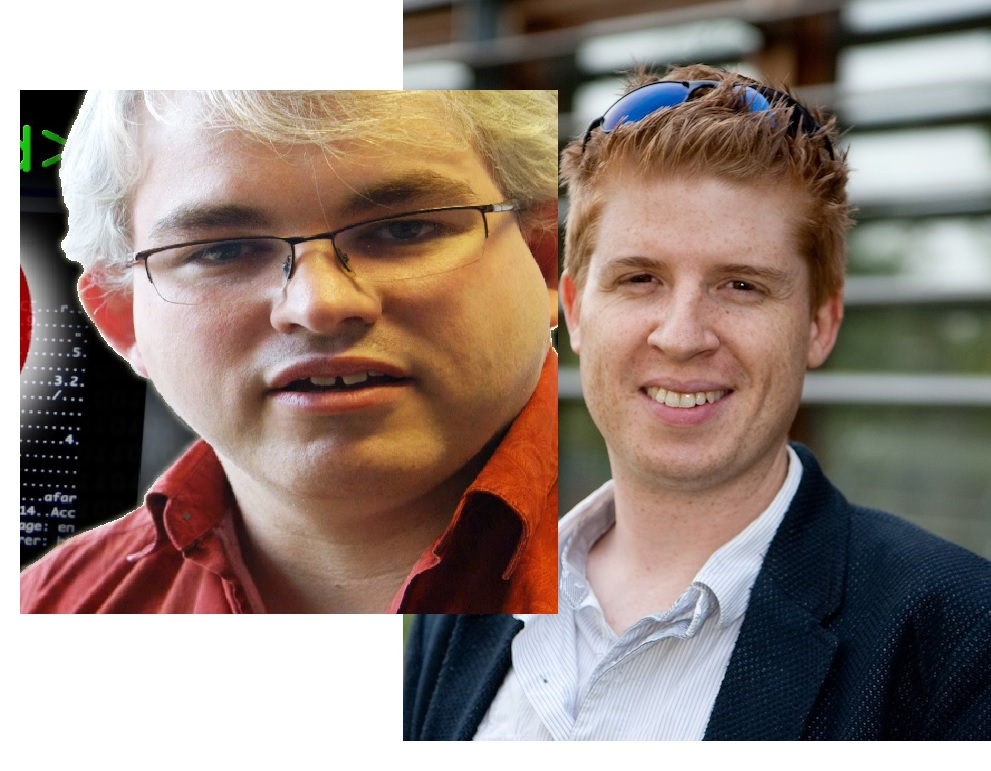
\includegraphics[width=0.5\textwidth]{selfieWithMax}
	\label{fig:selfie}
\end{figure}

My selfie with Max is in  Figure~\ref{fig:selfie}.

\subsection{What I have learned in this module}
I have learnt the importance of working in a team and that communication is key to be able to successfully complete the lab assignments. 

